\chapter{Methodology}\label{chap:methods}
In this chapter, the methodology to establish an accurate data basis is discussed.  Section \ref{subsec:hardware} describes the various pieces of hardware with their technical features, as well as the physical implementation in the actual experimental environment. The specific software infrastructure used to extract the information from the hardware is described in detail in section \ref{subsec:software}


\section{Measurement Equipment}
In this section, the actual implementation of the experiment is described in detail. The subsection \ref{subsec:hardware} details a description of the sensors, network equipment and server systems utilized during research. In subsection \ref{subsec:software} the structure, functionality and communication of all software components can be examined.
\subsection{Hardware}\label{subsec:hardware}
To collect relevant power data in the IT environment, an assortment of independently functional sensors was deployed.
The Allnet sensor units contain a linear hall sensor, which is able to measure consumption of appliances, as well as possible power provided by energy sources to the grid. All sensor units were evenly places into workplaces throughout the university facility. A schematic overview of all rooms and their workplace typification can be seen in figure \ref{fig:schema}.
\begin{figure}[h]
	\centering
	\includegraphics[width=\textwidth]{images/room_schematic.png}
	\caption{Room schematic of the office section of the university building.}
	\label{fig:schema}
\end{figure} 
An additional caveat of linear sensors is bias/noise in the sensor data can lead to negative values although the specific appliance is unable to work as an actual energy source. In the data set these 'erroneous' data points are not altered, as for example with the usage of battery equipped laptops, a short term negative consumption cannot be ruled out completely.\\
This way a (un-)conscious skew towards certain data trends by the experiment can be excluded. In table \ref{tab:allnet_data} a short overview of technical properties of the specific sensor model can be seen.

\begin{table}[b]
    \centering
    \begin{tabular}{cc}
    \hline
        supported voltage & 100-230V AC \\
        \hline
        max relay current & 8 ampere \\
        \hline
        operation temperature & 0-40 C°\\
        \hline
        Networking & IEEE 802.3u IEEE 802.11b/g/n\\
        \hline
    \end{tabular}
    \caption{technical data according to the manufacturer}
    \label{tab:allnet_data}
\end{table}

\subsubsection{Operation}
The configuration of a sensor, using factory settings, requires a computer with an Ethernet port, power supply, Ethernet cable, and a browser. As a short overview each configuration of the sensors  broadly follow the steps listed below:

\begin{enumerate}
	\item Connect the Allnet sensor via Ethernet to the computer.
	\item Configure your Ethernet port to populate the same subnet as the default address space of the sensor. (IPv4 192.168.0.100 by default) 
	\item Open browser and connect to the sensor using HTTP protocol. 
	\item Follow the instructions given by the device.
	\item Configure network settings according to the local are network the sensor should be integrated in.
	\item Restart device to update network configuration.
\end{enumerate}

\subsubsection{Data Access}
The internal Unix server provides different data accesses for both actuators and sensors via an REST API system in JSON and XML format.
The relevant structure of the REST addresses can be seen in listing \ref{lst:allnet_rest}.

    \begin{lstlisting}[language=python, caption={address format of a sensor, provided variable values of a valid ip\_address (0.0.0.0 to 255.255.255.255) a format (xml or json) and a valid mode (all, sensor, ).},label={lst:allnet_rest}]
rest_address = f"http://{ip_address}/{format}/?mode={mode}"
\end{lstlisting}

At the setup of the experiment, the provided batch of sensors did not transmit sensory data via the JSON format, therefore the measurements were taken using the XML data provided. An exemplary data item with structure description can be seen in figure \ref{fig:xml_data}.
To determine which values are provided, the mode parameter can be chosen to include sensory data only, actuators only, or all. It is necessary to enable remote access to the device using the HTML interface of the sensor. After successful initialization, current sensory data readings can be accessed using the REST API of the device. The result of each HTML request is a response in the data format specified in the 'format' parameter.
\newpage

\begin{lstlisting}[language=xml, caption={Example data item from a power measurement}, label={fig:xml_data}]
<?xml version="1.0" encoding="UTF-8"?>
<sensors>
 <sensor>
   <id>2</id>
   <name>AC Voltage</name>
   <current>227.25</current>
   <unit>V</unit>
   <minmax>
    <today>
     <min>
      <value>222.50</value>
      <date>03.08.2022 09:31:58</date>
      <timestamp>1659511918</timestamp>
      </min>
     <max>
      <value>233.95</value>
      <date>03.08.2022 05:01:24</date>
      <timestamp>1659495684</timestamp>
      </max>
     </today>
     <absolute>
      <min>
       ...
      </min>
      <max>
       ...
      </max>
     </absolute>
    </minmax>
  </sensor>
  <sensor>
    ...
  </sensor> ...
\end{lstlisting}

The parsing of each XML data package is done by the software running in the 'Pika Producer' service which is further described in section \ref{subsec:software}.
\\
To connect all measurement devices, a wireless local area network was configured using a FRITZ!Box 7590, latest running on FRITZ!OS version 7.29.
As the router is located behind a well secured university firewall, a fitting setup had to be found. 
The access to each individual sensor had to be configured using port forwarding to access the router's subnet and exposing the host into the university intranet. To access any part of the docker software running on the virtual machine, an access via the university network or VPN is strictly necessary to avoid compromising any it security. As any connection using wireless connections is more susceptible to distortions, the evaluation tables contained a measurement to be able to evaluate unexpected values due to a lack of measurements in the future. The minimum number of measurement counts can reach low single digits, although the average for all tables is around the high 70s. The exact measurements can be seen in table \ref{tab:counts}, which provide a confident basis for evaluation.

\begin{table}
	\centering
	\begin{tabular}{l|c}
		Table & Count \\
		\hline
		 Sensor\_1\_Meta  & 90\\ \hline
		 Sensor\_2\_Meta  & 70\\ \hline
		 Sensor\_3\_Meta  & 90\\ \hline
		 Sensor\_4\_Meta  & 85\\ \hline
		 Sensor\_5\_Meta  & 80\\ \hline
		 Sensor\_6\_Meta  & 77\\ \hline
		 Sensor\_7\_Meta  & 71\\ \hline
		 Sensor\_8\_Meta  & 86\\ \hline
		 Sensor\_9\_Meta  & 84\\ \hline
		 Sensor\_10\_Meta  & 89\\ \hline
		 Sensor\_11\_Meta  & 90\\ \hline
		 Sensor\_12\_Meta  & 90\\ \hline
		 Sensor\_13\_Meta  & 89\\ \hline
		 Sensor\_14\_Meta  & 90\\ \hline
		 Sensor\_15\_Meta  & 90\\ \hline
		 Sensor\_16\_Meta  & 90\\ \hline
		 Sensor\_17\_Meta  & 90\\ \hline
		 Sensor\_18\_Meta  & 90\\ \hline
		 Sensor\_19\_Meta  & 89\\ \hline
		 Sensor\_20\_Meta  & 90\\ \hline 
		 Sensor\_21\_Meta  & 90\\ \hline
		 Sensor\_22\_Meta  & 90\\ \hline
		 Sensor\_23\_Meta  & 90\\ \hline
		 Sensor\_24\_Meta  & 89\\ \hline
		 Sensor\_25\_Meta  & 90\\ \hline
		 Sensor\_26\_Meta  & 89\\ \hline
		 Sensor\_27\_Meta  & 90\\ \hline
		 Sensor\_28\_Meta  & 90\\ \hline
		 Sensor\_29\_Meta  & 90\\ \hline
		 Sensor\_30\_Meta  & 88\\ \hline
		 Sensor\_31\_Meta  & 90\\ \hline
		 Sensor\_32\_Meta  & 90\\ \hline
		 Sensor\_33\_Meta  & 90\\ \hline
		 Sensor\_34\_Meta  & 90\\ \hline
		 Sensor\_35\_Meta  & 90\\ \hline
		 Sensor\_36\_Meta  & 90\\ \hline
	\end{tabular}
	\caption{average measurement count per 15 minute interval. Rounded to the full integer}
	\label{tab:counts}
\end{table}

\subsubsection{Virtual Machine}
To build the necessary infrastructure, host the database and run continuous software, the university provided access to a virtual Linux machine. The VM can be accessed in the university intranet using the URL 'energy.uni-passau.de'. Via this address, all software applications are made available using docker port forwarding. The address overview for access to all tools can be seen in table \ref{tab:access}. The service can be used by ordinary browsers using the base URL and the service port suffix, e.g. 'https://energy.uni-passau.de:3050'. These suffixes can be changed using the respective docker files of their services. For functionality of each service, refer to the respective section in \ref{subsec:software}.\\
In conclusion this setup allows an individual request to each sensor and the local subnet can be accessed by the virtual machine which is connected to the university intranet. Further information on the deployed software services can be found in the following section \ref{subsec:software}.
\begin{table}
\centering
\begin{tabular}{l|c}
	\hline
	Grafana & 3050 \\ \hline
	Adminer & 8181 \\ \hline
	PSQL DB & 6543 \\ \hline
	RabbitMQ & 8080
\end{tabular}
\caption{access ports for the respective docker services. Can be used as suffix after the url energy.uni-passau.de:'suffix'}
\label{tab:access}
\end{table}
\subsection{Software}\label{subsec:software}

The energy virtual machine is used by different members of the university chair. To avoid cluttering of the system, each piece of software is running in an isolated \gls{docker} image. Communication between the docker services is possible using docker bridges and connections from the outside are port forwarded from the VM to the docker host. An overview of all running docker services can be seen in figure \ref{fig:docker_overview}. The services are divided by functionality into Producer and Consumer Services. This relates to the nomenclature used in the context of message brokers. In the experiment the open source broker implementation Rabbit MQ is used and serves as the connection between producer and consumer services. Each group of services can be started at once by using the respective docker-compose file in each package.
\begin{figure}
	\centering
	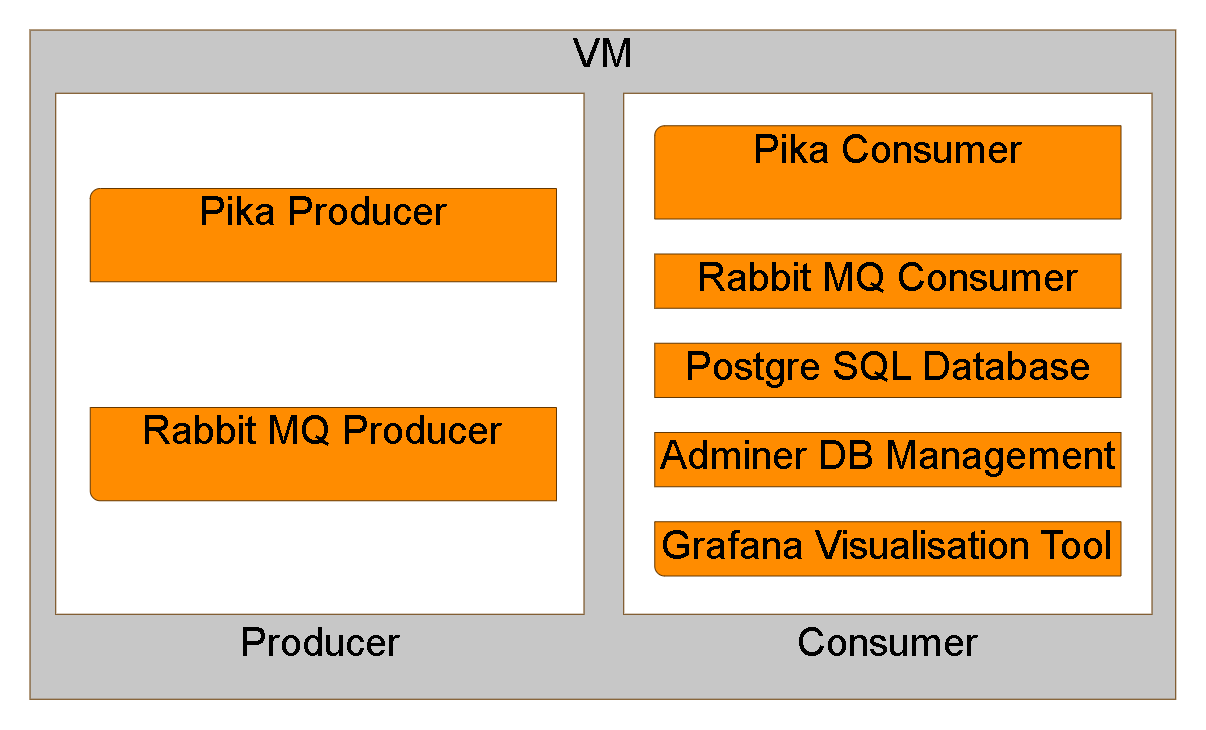
\includegraphics[width=\textwidth]{images/Docker_Services_Overview.png}
	\caption{Overview of active docker services within the docker VM}
	\label{fig:docker_overview}
\end{figure}
\subsubsection{Producer}
The task of the producer services is to provide sensory data received from individual requests to sensors in a consumable format. The producer service package is a continuation of the base skeleton provided by M. Sc. Sebastian Wilhelm (refer to the producer package in the repository \cite{wilhelm_repo}). Besides altering the operation mode from a distributed system using raspberry pis to a centralized vm structure, simplification of setup parameters, security and cryptography feature addition, https support, many automated recovery features, like retry loops, cleaning of faulty measurement readings were implemented.
\paragraph{Pika Consumer}  The consumer establishes a pool of threads establishing (secured, if enabled,) connections to each individual sensor. To avoid cluttering and overloading broker connections, separate existing measurement readings are pooled and released in chunks to the broker. Before transmission each xml response is parsed using the xml structure. The parsing is coded as such, to work with all similarly formatted files which are used by the manufacturer. That means the sensors which provide additional functionalities and sensory data can be seamlessly incorporated in the measurement.
Existing code and additional own contributions were commented to improve readability and maintenance.
The separate files are divided thus into their functionality:
\begin{tabular}{ll}
	AllnetPoll: & Provides the threading class and http request logic \\
	device\_name\_mapping: & defines and maps each sensor address to their respective\\ & table name \\
	local\_config: & enables the usage of subgroups of a bigger system by \\& limiting the number/range of addresses \\
	pika\_producer: & main class that initiates the threads, initiates pooling the\\ & measurements, and parses the packages \\
	pooling: & holds the round robin pool logic and determines chunk size.	\\
\end{tabular}\\

Additional files in the package only hold function for specific circumstances like operation on windows, or other setup prototypes for reference.

\paragraph{Rabbit MQ producer} is the producer instance of the rabbit mq message broker system. It enables asynchronous messaging between producer and consumer. This conversion step could strictly be bypassed, and is as such not necessary. This would be at the cost of modular structure, as this way provides the opportunity to run the respective instances of producer and consumer on different machines. The configuration of communication between docker images is the exact same was as communication via networking, and is therefore suitable for every kind of setup. The producer services provide their data to the docker host system. Via a docker bridge a DNS based connection can be established using docker image names or their respective address which are configured in the docker-compose file and the respective .env file of the producer. After successful setup the consumer can be established to receive incoming data. A comprehensive illustration of the information flow of the producer services can be seen in figure \ref{fig:information_flow_producer}.

\subsubsection{Consumer}
 In this package the counter parts of the producer elements can be instantiated. Besides similar configuration improvements, as made with the producer package, a second layer of fault detection to avoid null values was added. Different steps that became redundant due to simplification have been removed, like setup wait time that were accounted for in previously distributed networks. To depict the inner workings of the services it is important to note that within the consumer two separate functionalities should be differentiated. The services 'Pika Consumer', 'Rabbit MQ Consumer' and 'PostgreSQL Database' complete the functionality of record keeping. To simply save measurements to a database, these software packages will suffice. These three consumer services are built a continuation of the base skeleton provided by M. Sc. Sebastian Wilhelm refer to the consumer package in the repository \cite{wilhelm_repo}. Adminer and Grafana are simply additional tools for database management and visualizations and can be omitted if the respective application does not require such a step. Via docker compose functionality it is possible to add these functionalities into an already running recording tool.

\paragraph{Pika Consumer} receives incoming packages from the Rabbit MQ Consumer and saves them into the database via extracting messages into python dictionaries and inserting into,or respectively creating tables using the sqlalchemy library after a short fault check. For compatibility and maintenance reasons, all further evaluations, insertions and queries by code are also made using sqlalchemy. 

\paragraph{Rabbit MQ Consumer} acts as the counterpart to the Rabbit MQ Producer and only receives incoming parsed measurements. Connection configuration is made using environment variables in the .env file
	
\paragraph{PostgreSQL Database} is a docker image of an ordinary PostgreSQL database implementation. Connection configuration is made using environment variables in the .env file. Besides the tables created by the consumer, the active service also holds all metadata tables created during the evaluation phase described in section \ref{chap:results}. A short overview of the database tables, and their logic can be seen in figure \ref{db_tables}

\begin{figure}[ht]
	\centering
	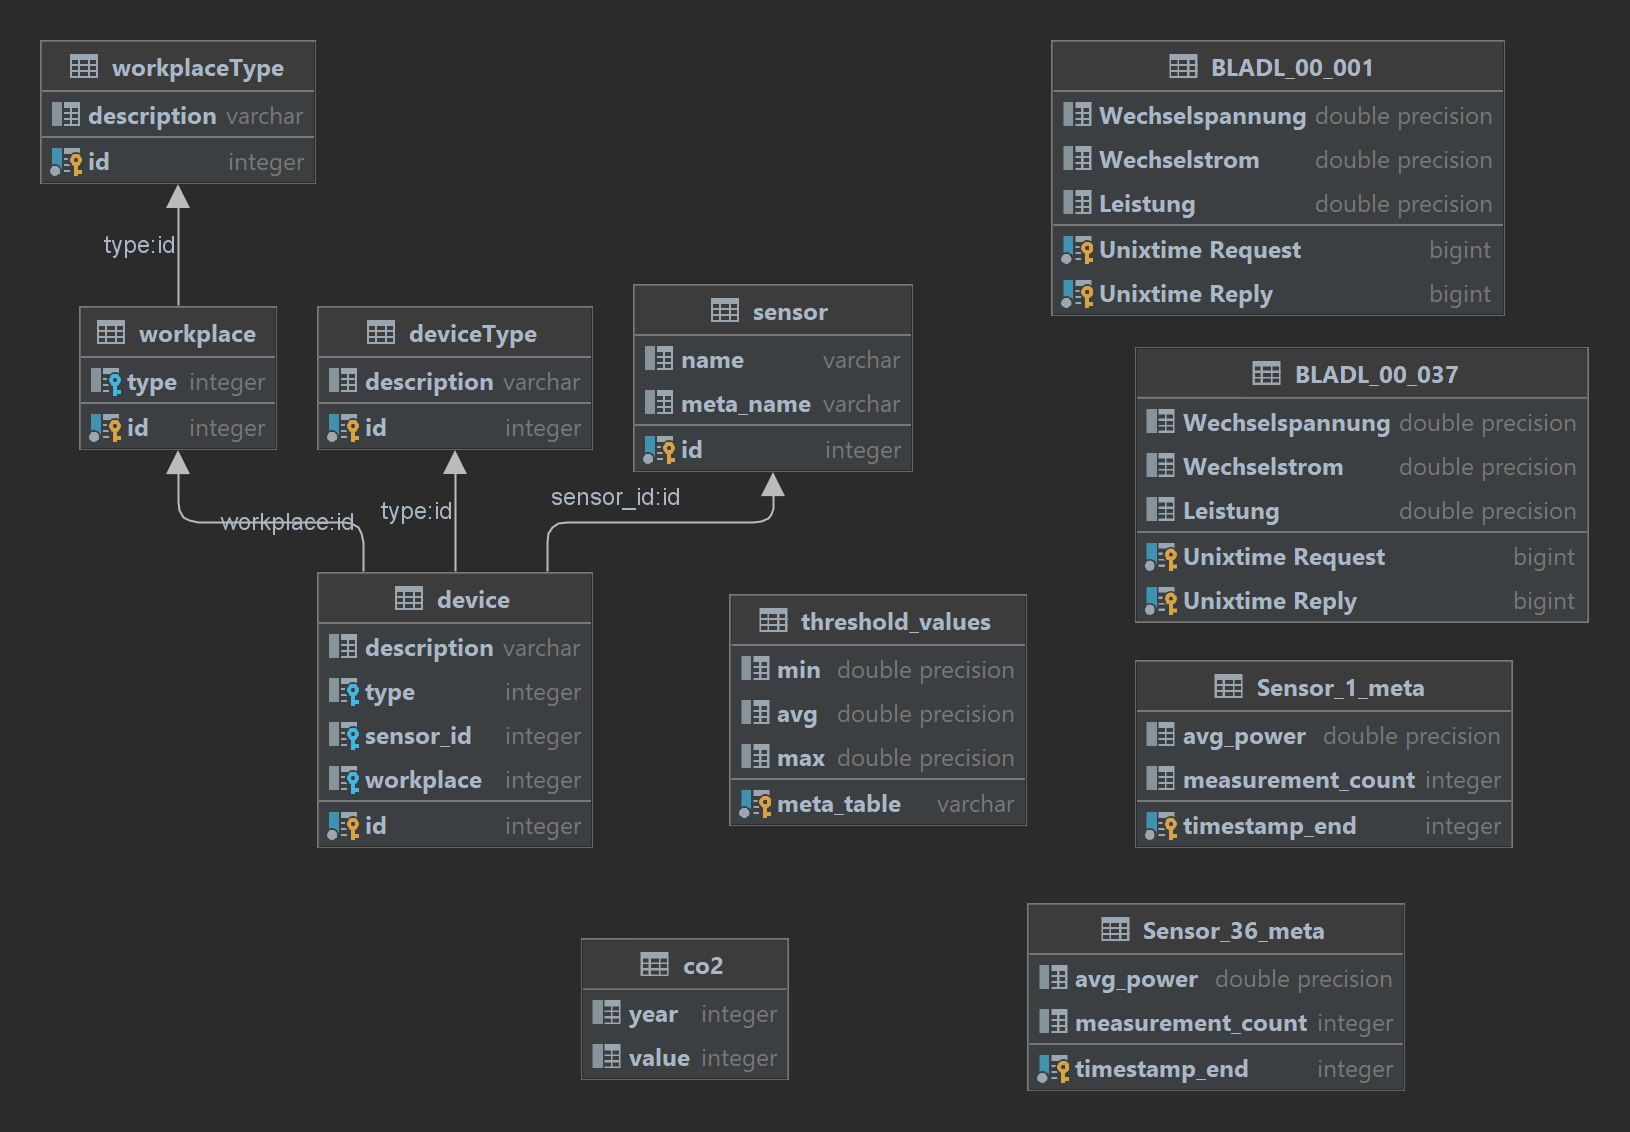
\includegraphics[width=\textwidth]{images/diagram.png}
	\caption{Overview of the different database tables. Foreign keys are marked, other concatenations are made using table names or dates. For simplicity, multiples of the measurement and meta tables are omitted}
	\label{db_tables}
\end{figure}

\paragraph{Grafana} is a time series visualization tool, to create interactive dashboards of a variety of data sources, including PostgreSQL. It provides many useful tools besides time series illustrations, like annotation capabilities, a user management system, and extensive query variables. A basic example dashboard which can be used to illustrate the data set of this work is described in the section \ref{subsec:RPMT}.

\paragraph{Adminer DB Management} is a lightweight administration tool for relational database systems. As the PostgreSQL service is usable like any other db system, any management tool of choice can also be used. However with this service an available management tool can be easily provided. A comprehensive illustration of the information flow of the consumer services can be seen in figure \ref{fig:information_flow_consumer}.\\
In combination, all services build a powerful foundation to manage, explore and evaluate a variety of datasets in energy consumption measurement. As part of the result section of this work, an example application, called \acrfull{rpmt}, is shown in section \ref{subsec:RPMT}

\begin{figure}
    \centering
    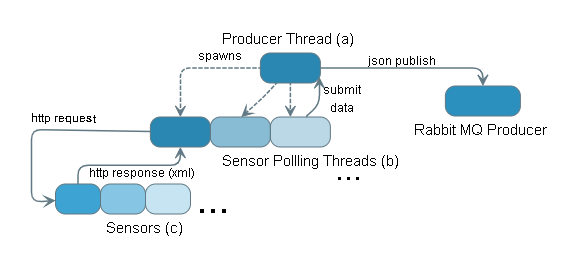
\includegraphics[width=\textwidth]{images/producer_flow.png}
    \caption{Information Flow Producer Service}
    \label{fig:information_flow_producer}
\end{figure}

\begin{figure}
    \centering
    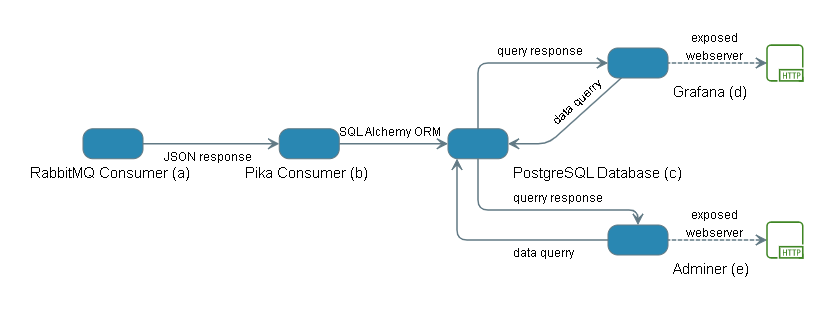
\includegraphics[width=\textwidth]{images/consumer_flow.png}
    \caption{Information Flow Consumer Service}
    \label{fig:information_flow_consumer}
\end{figure}

\subsubsection{Reference Measurement}
Besides the experimental measurements in the live office environment, an additional measurement using a single power consumer was undertaken. 
\paragraph{The setup} consists of a separate instance of all software components shown above, connected to a single power sensor identical to the other experiment. The reference device was chosen to produce similar power measurements over a longer period of time. As a suitable option, an actively cooled light source was chosen. Further technical details of the device can be seen in table \ref{tab:movinghead}.
\paragraph{The measurement} was taken for a total of 707063 seconds with around 20 000 individual measurements. To subtract interruptions due to setup time, all measurements near zero were eliminated. The clean data of the reference measurement can be seen in the \gls{main repo} as a CSV file. 
\paragraph{The resulting data set} was used as a basis for calculation of average values, maximum deviation, variance and standard deviation. The evaluation query can be seen in listing \ref{lst:eval}. Due to the results shown in table \ref{tab:result}, it can be assumed that individual measurements are accurate within about 1 watt. This correlates with values received from the measurement, which registered unused sockets at around -0.6 to 0.8 watts. As these deviations appear quite symmetrical, through the averaging process, these influences probably largely negate one another. However a precise measurement, where consumption and environmental variables are better controlled, could challenge this assumption. 

\begin{lstlisting}[language=sql, caption={Evaluation query of the reference measurement.}, label={lst:eval}]
	SELECT round(cast(avg("Leistung")as numeric),4) as "Average",
	round(cast(max("Leistung") - min("Leistung") as numeric),4) 
	as "Max-Deviation",
	round(cast(variance("Leistung") as numeric),4) as "Variance",
	round(cast(stddev("Leistung") as numeric),4) as "StdDev"
	FROM strommessung_1
	WHERE "Leistung" > 0
\end{lstlisting}

\begin{table}[h]
	\centering
	\begin{tabular}{cccc}
		Average &Max-Deviation &Variance &StdDev\\
		41.9417 &4.7 &0.7585 &0.8709
	\end{tabular}
	\caption{Result of the evaluation query in listing \ref{lst:eval}}
	\label{tab:result}
\end{table}

\begin{figure}
	\centering
	\begin{tabular}{l|c}
		\hline
		Model & MX-H25 LED Spotlight\\ \hline
		Manufacturer & Stairville\\ \hline
		Voltage & 230V\\ \hline
		Consumption (max) & 102W\\ \hline
		Operation Mode & Basic Mode b-CH\\ \hline
		
	\end{tabular}
	\caption{Excerpt from manufacturer specifications of the measured device}
	\label{tab:movinghead}
\end{figure}
\section{ \texorpdfstring{Evaluation Metrics/ \acrfullpl{kpi}}{Evaluation Metrics / KPI}}\label{sec:metrics}
To evaluate impacts on the environment a small set of well defined metrics is a useful tool. To give an easier overview of the difference in consumption between different devices, types, workplaces and users, this work supplies three distinct metrics represented in the evaluations or visualizations. 

\subsection{Idle Time of devices}\label{subsec:idle}
A core aspect of energy conservation is the avoidance of consumption all together. As a strong indicator of necessity the quantification of usage overall is already a great metric to evaluate a device. By the feasible measurement of machine usage, it should become easier to asses, if resources allocated to a workplace really rectify their existence. To refine this measurement a specific definition dependent on device type is advisable using external data, like validated expected usage data, or independent measurements like attendance can be useful. In this work idle time of a device is counted as the amount of time where data points in the respective 15 minute window do not exceed a value that is expected to be possible with only noise (+- 1 Watt). As different operation modes of devices, like standby, could also contribute as idle time in general, the results in this work should be considered a lower bound measurement of idle time. The mathematical formal definition of idle time can be seen in formula \ref{eq:idle}.
\begin{equation}\label{eq:idle}
	IDLE (X) = \sum x_j \bigg\rvert x_j \in X \wedge x_j < 1
\end{equation}
While in isolation this metric cannot be used to definitively determine proper usage of the device while energy is consumed, the lower bound of effective usage gained by the device can be established well. 
\subsection{ \texorpdfstring{\acrfull{wwcr}}{WWCR}}\label{subsec:wwcr}
As a second step of energy cost avoidance, the amount of ineffective electricity consumption should be established. To that idea, this work proposes a metric that is usable independently of other devices, and applicable to cases where energy consumption highly correlates with workload and usage. The ratio between the mean consumption over a \gls{workday} to the mean consumption over 24 hours will give information on the impact the user has on power consumption during working hours. In this context work hours are defined between 8am and 6pm during \glspl{workday}. Appliances like emergency lights will show no notable difference in \gls{workday} to weekday consumption. Although these device could contribute significantly to the energy total, no feasible direction to office staff could have a significant impact on this value. For a visual demonstration refer to figure \ref{fig:wwcr}. The specific idea is to reduce the area under the curve by reducing off work consumption, even at the cost of slight consumption increase during work hours. As electricity used while office appliances are not actively used, the identification, whether the device has potential in this regard is the value provided by this metric.
\begin{figure}[ht]
	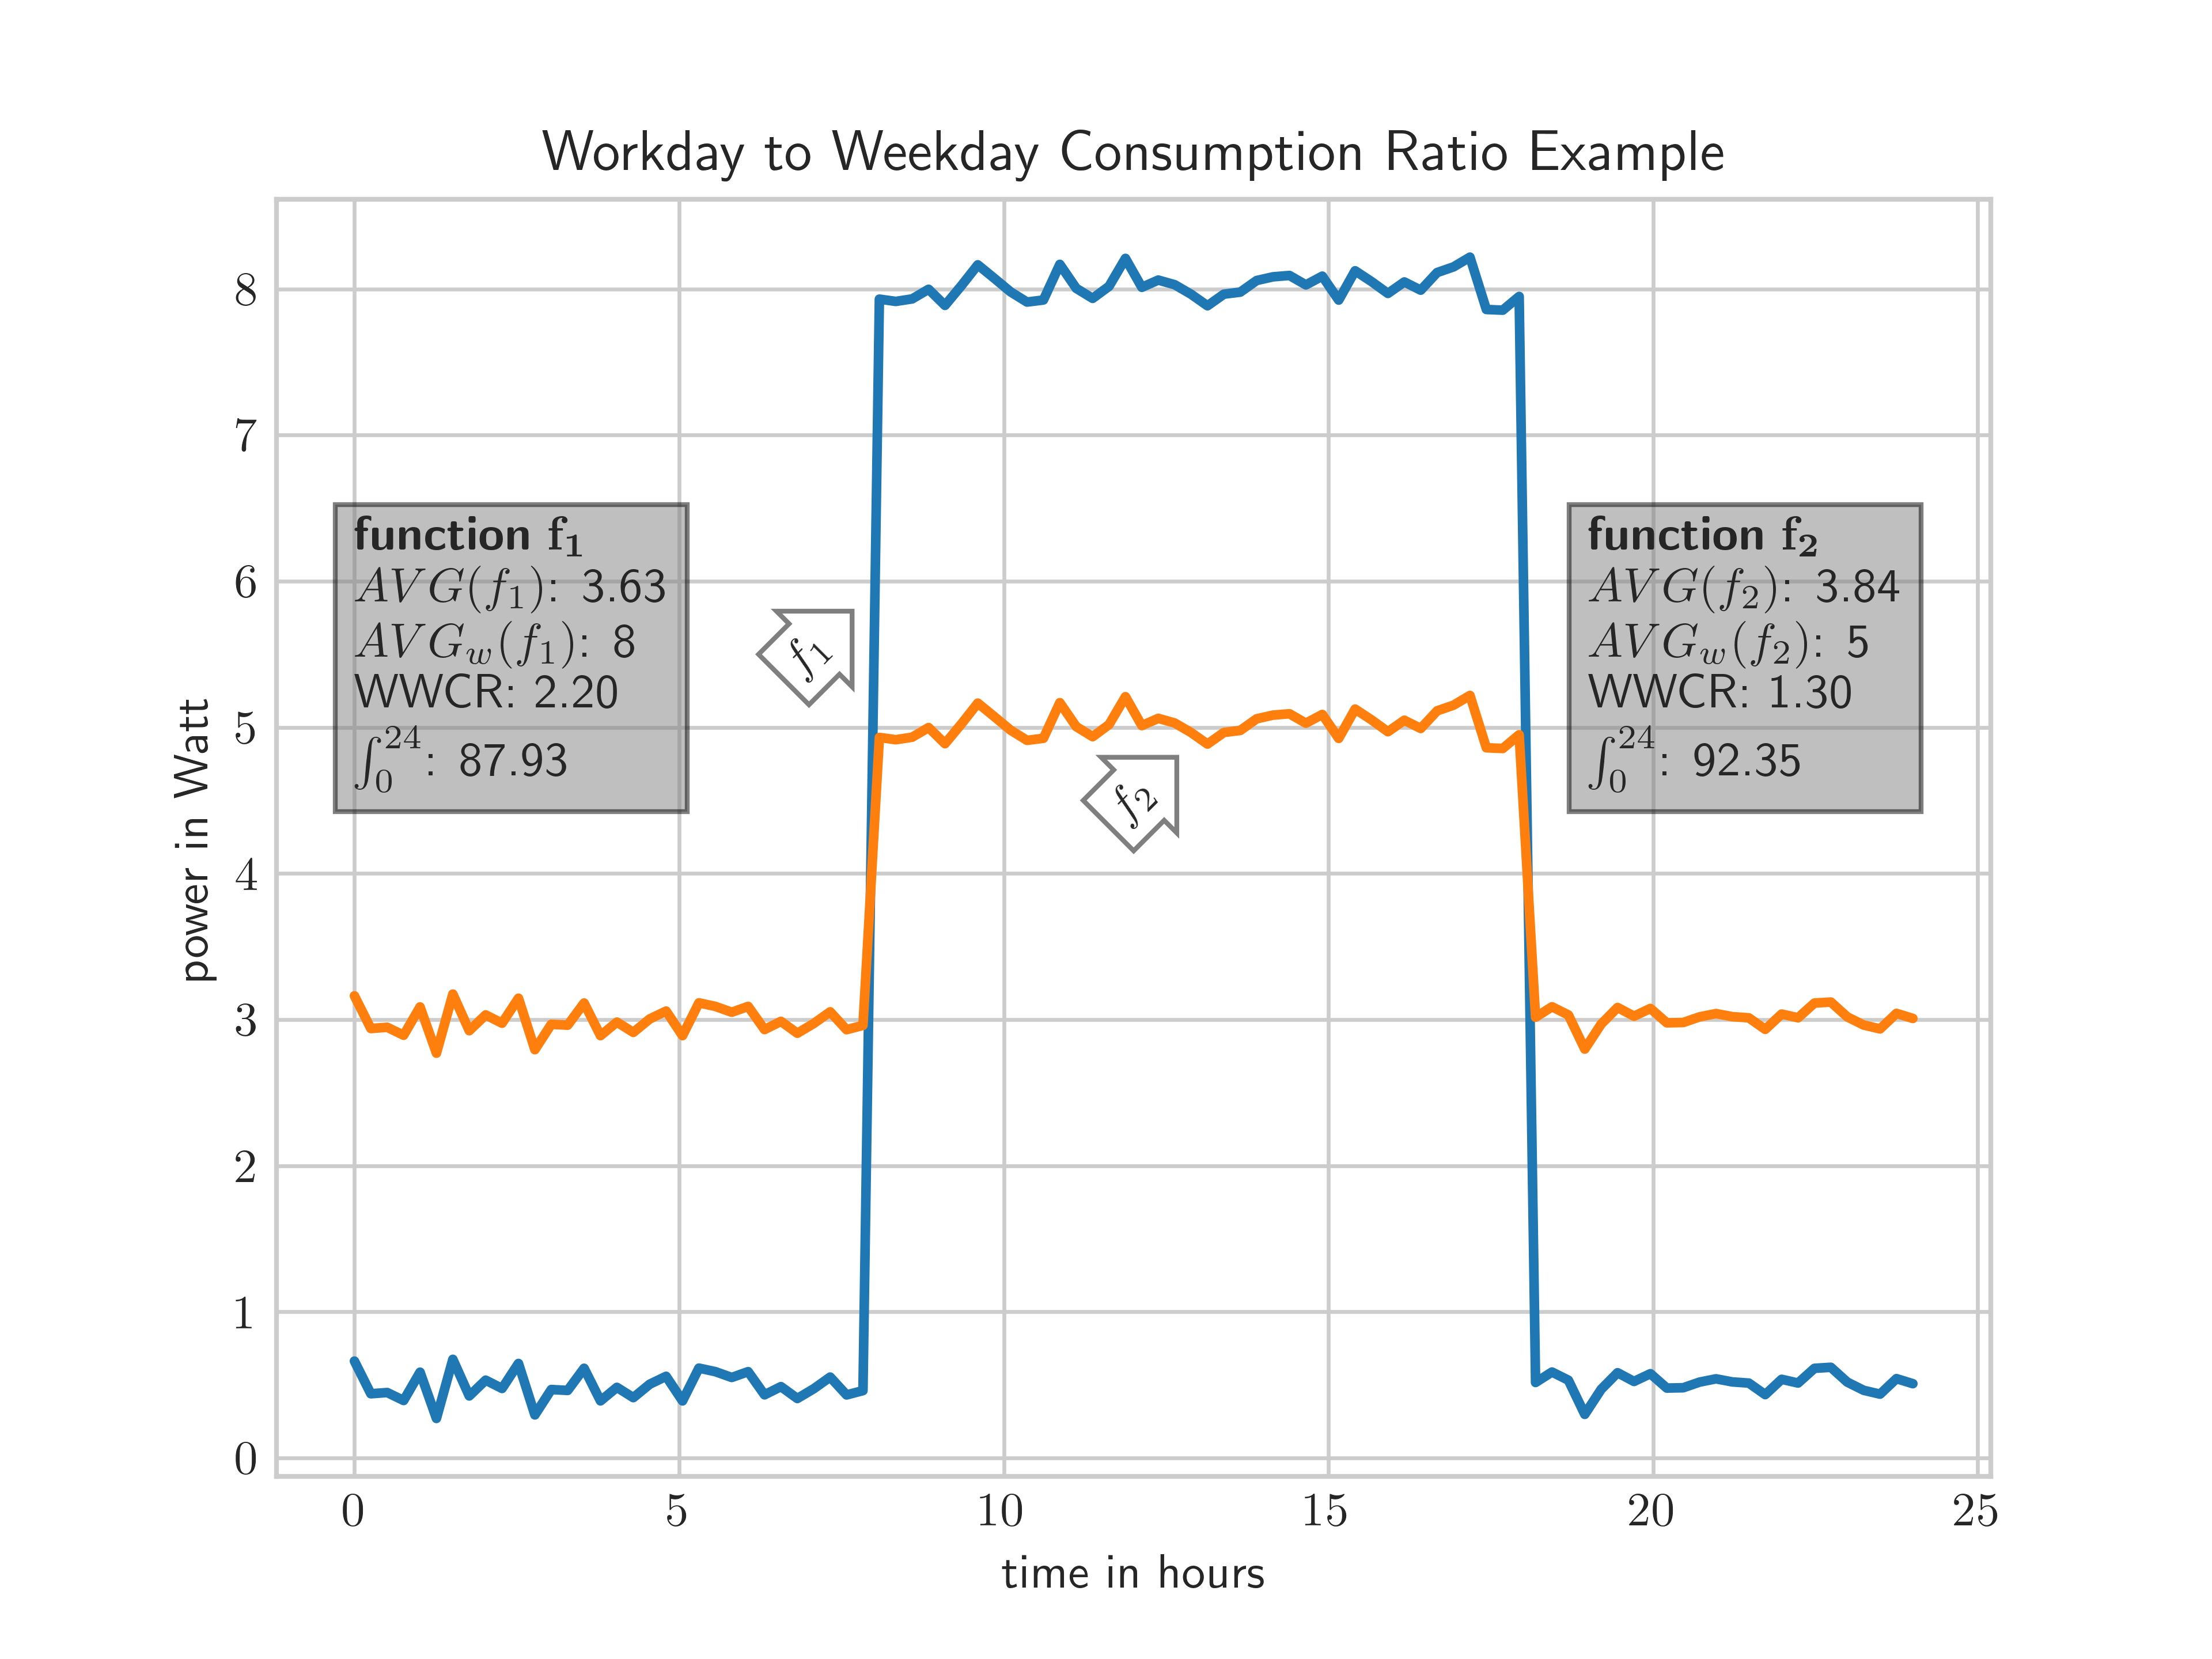
\includegraphics[width=\textwidth]{images/wwcr_plot.png}
	\caption{Example illustration of efficiency indication by \gls{wwcr}. By reducing energy wasted during off work time, the total consumption, which is the integral of the function curve, is reduced, even if working hour consumption is higher.}
	\label{fig:wwcr}
\end{figure}
Therefore a high WWCR indicates the possible impact any specific intervention on users could have. This establishes an objective possibility to rank office appliances on a sensitivity scale to avoid overwhelming staff members with diffuse worries about energy conservation. Actions taken can aim at narrow campaigns to conserve energy on specific devices, as goal specificity correlates to goal acceptance as shown in the literature \cite{steers}. Further than that, a low WWCR on unexpected devices, can give information on possibly wasted energy due to high or similar consumption outside of office hours. Refer to formula \ref{eq:wwcr} for calculation details. 
\begin{equation}\label{eq:wwcr}
	\begin{array}{l|l}
		\multirow{2}{*}{$WCR (X) = \dfrac{avg(X_w)}{avg(X)}$} & X \text{is a full weekday time series, }\\ & X_w\text{ subset of X during working hours} 
	\end{array}
\end{equation}
\subsection{ \texorpdfstring{CO$_2$ Footprint}{CO2 Footprint}}\label{subsec:footprint}
To determine an accurate CO$_2$ footprint of energy consumption a wide variety of methods can be used. One of the most widely used methods is depicted in section \ref{sec:co2works}, which unfortunately is unfit for the experiment. This is mainly due to the multitude of possible variables determining the exact amount of CO$_2$ emitted for the energy consumed. The accurate estimation of the CO$_2$ footprint created by energy used is a very elaborate process with several relevant factors provided by the power plant and the respective provider corporations. These figures are reported annually, and are not independent from foreign power generation influences.Besides the obvious co2 footprint of regional/national power generation, the actual ecological costs vary due to international power trading, governmental control over renewable energy supply and many more. The specific numbers for the visualizations of this work refer to the official European Environment Agency, made public in a csv data set \cite{co2_footprint}. On a national level, these number are available until the year 2020. These values show a very stable range due to a high rate of abstraction and averaging to reduce noise. The current calculation of the evaluation tool shown in section \ref{subsec:RPMT} uses a higher base value, as given by the source, due to two main factors. In 2020 a global short-term reduction in co2 emissions was registered, due to the pandemic \cite{NICOLINI2022154662}, and the previous downwards trend of co2 emissions is unlikely to persist. Furthermore persistent inflation in energy needs in Europe throughout 2022, as well as the dominance of coal-powered energy generation will further increase expected co2 emission intensity, as stated by the Statistisches Bundesamt publication "Pressrelease \#233 from 8 June 2022" \cite{destatista_coal}. As power generation with renewable energy sources rise simultaneously, and the respective European electricity footprint is lower than the domestic average, in this work the mean CO2 emission intensity of the years 2018 to 2020, which amounts to 356g of $CO_2$ per kWh, is considered a reasonable estimation, and has to be reevaluated when accurate values are available.